\iffalse
\documentclass[journal,10pt,twocolumn]{article}
\usepackage{graphicx, float}
\usepackage[margin=0.5in]{geometry}
\usepackage{amsmath, bm}
\usepackage{array}
\usepackage{booktabs}


\providecommand{\norm}[1]{\left\lVert#1\right\rVert}
\let\vec\mathbf
\newcommand{\myvec}[1]{\ensuremath{\begin{pmatrix}#1\end{pmatrix}}}
\newcommand{\mydet}[1]{\ensuremath{\begin{vmatrix}#1\end{vmatrix}}}

\title{\textbf{Circle Assignment}}
\author{Maddu Dinesh}
\date{September 2022}

\begin{document}

\maketitle
\paragraph{\textit{Problem Statement} -
\fi
Let $\angle PQR = 100\degree$ where $\vec{P}\vec{Q}, \vec{R}$ are points on a circle with centre $\vec{O}$. Find $\angle OPR$.
	\begin{figure}[!ht]
		\centering
 \includegraphics[width=\columnwidth]{chapters/9/10/5/3/figs/fig-1.pdf}
		\caption{}
		\label{fig:9/10/5/3}
  	\end{figure}
	\solution In Fig. 
		\ref{fig:9/10/5/3},
\begin{align}
	\vec{P} = \myvec{\cos\brak{\theta + 160} \\ \sin \brak{\theta + 160}}, \vec{Q} = \myvec{\cos \alpha\\ \sin \alpha}, \vec{R} = \myvec{\cos \theta \\ \sin \theta}.
\end{align}

\iffalse

\section*{\large Solution}

\begin{figure}[H]
\centering
\includegraphics[width=1\columnwidth]{fig-1.pdf}
\label{fig:triangle}
\end{figure}



Given  $\angle$PQR=100°





\section*{ Construction}






{
\setlength\extrarowheight{1pt}


\begin{tabular}{|c|c|c|}
 \hline
 \textbf{Symbol}&\textbf{Value}&\textbf{Description}\\
 \hline
 O&&Centre\\
 \hline
 $\angle$PQR&100$^\circ$&Angle between vectors P and R\\
 \hline
 $\angle$OPR&??&Angle b/w vectors O and R w.r.to P\\
 \hline
 
\end{tabular}

{


\section*{Proof:}
From assumptions the vector points P,Q,R be
\begin{eqnarray}
 \vec{P} = \myvec{cos\theta_1\\sin\theta_1},
 \vec{Q} = \myvec{cos\theta_2\\sin\theta_2},
 \vec{R} = \myvec{cos\theta_3\\sin\theta_3},
 \vec{O} = \myvec{0\\0}
\end{eqnarray}

\begin{align}
 cos(\angle PQR) = \frac{(P-Q)^T(R-Q)}{\norm{P-Q}\norm{R-Q}}
 \label{pf2-eq-1}
\end{align}

Where
 \begin{eqnarray}
 \vec{P-Q} = \myvec{cos\theta_1 - cos\theta_2\\sin\theta_1 - sin\theta_2},
 \vec{R-Q} = \myvec{cos\theta_3 - cos\theta_2\\sin\theta_3 - sin\theta_2}
\end{eqnarray}
 

\begin{eqnarray*}
 (P-Q)^T(R-Q)=\myvec{cos\theta_1 - cos\theta_2  sin\theta_1 - sin\theta_2}
 \myvec{cos\theta_3 - cos\theta_2\\sin\theta_3 - sin\theta_2}
\end{eqnarray*}

\begin{multline*}
 = (\cos\theta_1-\cos\theta_2)(\cos\theta_3-\cos\theta_2)+(\sin\theta_1-\sin\theta_2)(\sin\theta_3-\sin\theta_2)
\end{multline*}

\begin{multline*}
 = -2\sin\frac{\theta_1-\theta_2}2\sin\frac{\theta_1+\theta_2}2 \cdot(-2)\sin\frac{\theta_3-\theta_2}2\sin\frac{\theta_3+\theta_2}2 \\\quad+ 2\cos\frac{\theta_1+\theta_2}2\sin\frac{\theta_1-\theta_2}2 \cdot 2\cos\frac{\theta_2+\theta_3}2\sin\frac{\theta_3-\theta_2}2
\end{multline*}
\begin{multline*}
 = 4\sin\frac{\theta_1-\theta_2}2\sin\frac{\theta_3-\theta_2}2(\sin\frac{\theta_1+\theta_2}2\sin\frac{\theta_3+\theta_2}2+\\
 \cos\frac{\theta_1+\theta_2}2\cos\frac{\theta_3+\theta_2}2)
\end{multline*}
\begin{align*}
 = 4\sin\frac{\theta_1-\theta_2}2\sin\frac{\theta_3-\theta_2}2\cos\left(\frac{\theta_1+\theta_2}2-\frac{\theta_3+\theta_2}2\right)
\end{align*}
\begin{align}
 = 4\sin\frac{\theta_1-\theta_2}2\sin\frac{\theta_3-\theta_2}2\cos\frac{\theta_1-\theta_3}2
 \label{pf2-eq-2}
\end{align}

\begin{multline*}
 \norm{P-Q}^2\norm{R-Q}^2 = ((\cos\theta_1-\cos\theta_2)^2+(\sin\theta_1-\sin\theta_2)^2)\\
 ((\cos\theta_3-\cos\theta_2)^2+(\sin\theta_3-\sin\theta_2)^2)
\end{multline*}
\begin{multline*}
 = (2-2\cos\theta_1\cos\theta_2 - 2\sin\theta_1\sin\theta_2)(2-\\
 2\cos\theta_3\cos\theta_2 - 2\sin\theta_3\sin\theta_2)
\end{multline*}
\begin{align*}
 &= 16 \sin^2\frac{\theta_1-\theta_2}2\sin^2\frac{\theta_3-\theta_2}2
\end{align*}
\begin{align}
 \norm{P-Q}\norm{R-Q} = 4 \sin\frac{\theta_1-\theta_2}2\sin\frac{\theta_3-\theta_2}2
 \label{pf2-eq-3}
\end{align}

Substituting (\ref{pf2-eq-2}) and (\ref{pf2-eq-3}) in (\ref{pf2-eq-1}),
\begin{multline*}
 cos(\angle PQR) = \frac{4sin\frac{\theta_1-\theta_2}{2}sin\frac{\theta_3-\theta_2}{2}cos\frac{\theta_1-\theta_3}{2}}{4 \sin\frac{\theta_1-\theta_2}2\sin\frac{\theta_3-\theta_2}2}
\end{multline*}
\begin{equation}
cos(\angle PQR) = cos\frac{\theta_1-\theta_3}{2}
\label{pf2-eq-4}
\end{equation}
\begin{equation*}
\angle PQR = =\frac{\theta_1 - \theta_3 }{2}=100^\circ
\end{equation*}


\begin{align}
 cos(\angle OPR) = \frac{(P-R)^T(P-O)}{\norm{P-R}\norm{P-O}}
 \label{pf2-eq-5}
\end{align}

\begin{eqnarray}
 \vec{P-R} = \myvec{cos\theta_1 - cos\theta_3\\sin\theta_1 - sin\theta_3},
 \vec{P-O} = \myvec{cos\theta_1 \\sin\theta_1 }
\end{eqnarray}
 

\begin{eqnarray*}
 (P-R)^T(P-O)=\myvec{cos\theta_1 - cos\theta_3\\sin\theta_1 - sin\theta_3}
 \myvec{cos\theta_1 sin\theta_1 }
\end{eqnarray*}

\begin{multline*}
 = (\cos\theta_1-\cos\theta_3)(\cos\theta_1)+(\sin\theta_1-\sin\theta_3)(\sin\theta_1)
\end{multline*}
\begin{multline*}
 = (\cos^2{\theta_1}-\cos\theta_3\cos\theta_1)+(\sin^2{\theta_1}-\sin\theta_1\sin\theta_3)
\end{multline*}
\begin{align*}
 = 1-(\cos\theta_3\cos\theta_1+\sin\theta_1\sin\theta_3)
\end{align*}
\begin{equation}
=1-(cos(\theta_3-\theta_1))
\end{equation}
\begin{multline*}
 \norm{P-R}^2\norm{P-O}^2 = ((\cos\theta_1-\cos\theta_3)^2+(\sin\theta_1-\sin\theta_3)^2)\\
 ((\cos\theta_1)^2+(\sin\theta_1)^2)
\end{multline*}
\begin{align*}
 = 2-2\cos\theta_1\cos\theta_3-2\sin\theta_1\sin\theta_3
\end{align*}
\begin{align*}
 = 2(1-\cos(\theta_1-\theta_3) )
\end{align*}
\begin{align}
 \norm{P-R}\norm{P-O} = \sqrt{2(1-\cos(\theta_1-\theta_3))}
 \label{pf2-eq-6}
\end{align}
\begin{align*}
 cos(\angle OPR) = \frac{(1-\cos(\theta_1-\theta_3)) }{\sqrt{2(1-\cos(\theta_1-\theta_3))}}
\end{align*}
\begin{align*}
\cos(\angle OPR)=0.98
\end{align*}
\begin{align}
\angle OPR=10^\circ
\end{align}






\end{document}
Footer
\fi
